\documentclass{article}
\usepackage{tikz}
\usetikzlibrary{trees}

\begin{document}

\section{Description of the problem}
We're placed in a room of size $10 \times 10$, we're surrounded by walls, and
we know that there's exactly $1$ secret door hidden in a wall. Performing a
research on a square will reveal a secret door in one of the neighboor squares
with a probability of $\frac{1}{7}$ if the secret door is among the neighboors.
\\
Here's a view of what the map looks like, violet squares being the location
where a secret door might be found.


\begin{center}
  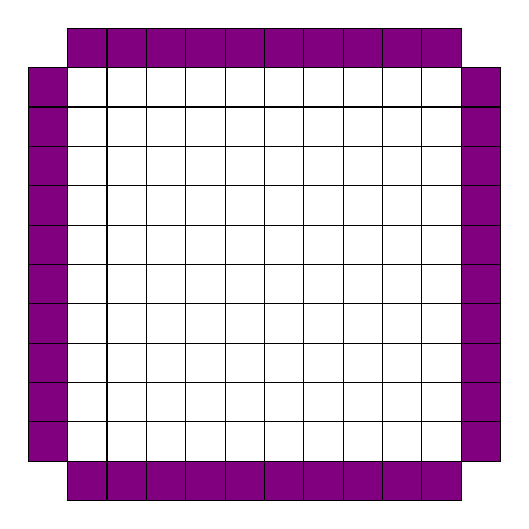
\begin{tikzpicture}[scale=.5]
    % Drawing Walls part
    \foreach \x in {1,...,10}{
      \draw [fill=violet] (\x,  0) rectangle (\x + 1,  1);
      \draw [fill=violet] (\x, 11) rectangle (\x + 1, 12);
    }
    \foreach \y in {1,...,10}{
      \draw [fill=violet] ( 0, \y) rectangle ( 1, \y + 1);
      \draw [fill=violet] (11, \y) rectangle (12, \y + 1);
    }
    % Drawing internal grid
    \foreach \x in {1,...,10}{
      \foreach \y in {1,...,10}{
        \draw (\x,\y) rectangle (\x + 1,\y + 1);
      }
    }
  \end{tikzpicture}
\end{center}

Being sure that we have the best solution to the problem can be quite tricky,
that is the reason why we will try to find a lower bound as first objective.
Once one has been found, we can compare it with our bots results. At the same
time, we can try to :
\begin{itemize}
\item Increase the lower bound with some theoric addition
\item Decrease the upper bound by improving the bot
\end{itemize}

\section{Dominating the room}
It is possible to fix some squares where research would be performed, trying to
use the lowest number of squares and avoiding two possible research on the
same square \footnote{This notion is close to the notion of domination set in
graph theory}. We can then obtain following result, with the filled orange
squares being the squares where research would be performed. And the empty
orange squares being the range of research.

\begin{center}
  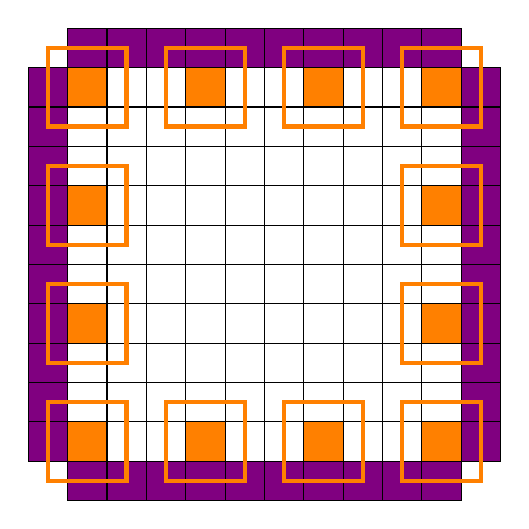
\begin{tikzpicture}[scale=.5]
    % Drawing Walls part
    \foreach \x in {1,...,10}{
      \draw [fill=violet] (\x,  0) rectangle (\x + 1,  1);
      \draw [fill=violet] (\x, 11) rectangle (\x + 1, 12);
    }
    \foreach \y in {1,...,10}{
      \draw [fill=violet] ( 0, \y) rectangle ( 1, \y + 1);
      \draw [fill=violet] (11, \y) rectangle (12, \y + 1);
    }
    % Drawing internal grid
    \foreach \x in {1,...,10}{
      \foreach \y in {1,...,10}{
        \draw (\x,\y) rectangle (\x + 1,\y + 1);
      }
    }
    % Coloring squares and ranges of research
    \foreach \x in {1,4,7,10}{
      \draw [fill=orange] (\x,  1) rectangle (\x + 1,  2);
      \draw [fill=orange] (\x, 10) rectangle (\x + 1, 11);
      \draw [ultra thick, orange] (\x - 0.5, 0.5) rectangle (\x + 1.5,  2.5);
      \draw [ultra thick, orange] (\x - 0.5, 9.5) rectangle (\x + 1.5, 11.5);
    }
    \foreach \y in {1,4,7,10}{
      \draw [fill=orange] ( 1, \y) rectangle ( 2, \y + 1);
      \draw [fill=orange] (10, \y) rectangle (11, \y + 1);
      \draw [ultra thick, orange] (0.5, \y - 0.5) rectangle ( 2.5, \y + 1.5);
      \draw [ultra thick, orange] (9.5, \y - 0.5) rectangle (11.5, \y + 1.5);
    }
  \end{tikzpicture}
\end{center}
Obviously, it's impossible to cover each square with a potential secret door
with less squares, because all the corners are used and there isn't any square
being ``covered'' by two different squares. If we ignore the cost of moves,
considering only the cost of research, the best policy seems to be always
looking first in the corners and after in the other spots, if all have the same
number of research at starts. But it's not obvious that the chance of finding a
secret door in a corner with $n+1$ researches is always lower than the chance
of finding a secret door in a wall with $n$ researches.

\section{Probabilities to found the doors}
The initial probability of founding a secret door is equal to
$\frac{1}{40} \times \frac{1}{7}$, the initial probability of founding a secret
door is then $4 \times \frac{1}{40} \times \frac{1}{7}$. Through the research,
the $\frac{1}{7}$ part (representing the probability of finding the secret door
knowing that the secret door is here) will stay stable. But the probability
that the secret door is in a specific square will change depending on the
number of research will change\footnote{The problem presented here is a variant
of the famous 3-doors problems because we \emph{know} that there's one door
among the forty squares}.\\
An intuition of this fact can be found in the following example : 10'000
thousands research have been done on every research spot but the top-left
corner where no research has been done, it seems very likely that the secret
door is located in one of the squares covered by the top-left corner.

\subsection{Seeing it as a probability tree}
Before drawing this situation as a probability tree, we can simplify the
problem by saying that there's only 2 squares where a door could be and each
research can try only one of those squares.
We can then get the following tree after one research on position $1$.
\begin{itemize}
\item $Pos(D)$ is the position of the door.
\item $F$ means door has been found
\item $NF$ means nothing has been found
\end{itemize}
% Set the overall layout of the tree
\tikzstyle{level 1}=[level distance=3.5cm, sibling distance=3.5cm]
\tikzstyle{level 2}=[level distance=3.5cm, sibling distance=2cm]

% Define styles for bags and leafs
\tikzstyle{bag} = [text width=4em, text centered]
\tikzstyle{end} = [circle, minimum width=3pt,fill, inner sep=0pt]
\begin{center}
  \begin{tikzpicture}[grow=right, sloped]
    \node[bag] {Overall}
    child {
      node[bag] {Door in $1$}        
      child {
        node[end, label=right:
          {If we reach this point, game is stopped}] {}
        edge from parent
        node[above] {$F$}
        node[below]  {$\frac{1}{7}$}
      }
      child {
        node[end, label=right:
          {$$}] {}
        edge from parent
        node[above] {$NF$}
        node[below]  {$\frac{6}{7}$}
      }
      edge from parent 
      node[above] {$Pos(D) = 1$}
      node[below]  {$\frac{1}{2}$}
    }
    child {
      node[bag] {Door in $2$}
      child {
        node[end, label=right:
          {$$}] {}
        edge from parent
        node[above] {$NF$}
        node[below]  {$1$}
      }
      edge from parent         
      node[above] {$Pos(D) = 2$}
      node[below]  {$\frac{1}{2}$}
    };
  \end{tikzpicture}
\end{center}

As a result of this tree, if the search on $1$ result with a $NF$, new
probabilities can be easily calculated :
\begin{itemize}
\item $P(Pos(D) = 1) = \frac{\frac{1}{2} \times \frac{6}{7}}
                            {\frac{1}{2} \times \frac{6}{7} +
                             \frac{1}{2}}
                     = \frac{6}{13}$
\item $P(Pos(D) = 2) = \frac{\frac{1}{2}}
                            {\frac{1}{2} \times \frac{6}{7} +
                             \frac{1}{2}}
                     = \frac{7}{13}$
\end{itemize}

\subsection{Another method}
We have already shown that the two location have not the same probability
anymore. It is also easy to see that calculating probabilities with this
method will be very difficult for a high number of research will be really
painful. This is why we tried to focus on another approach, easier to
calculate and faster to run on a computer.\\
Refering to the previous tree, it's easy to see that the probability that a
research on a square give a successful result depends only from the
probability that the door is effectively in this place.
\\
In order to solve this problem in a more generic way, we will define some
parameters used.
\begin{itemize}
\item $W$ is the set of all the squares which can contain a secret door:
  $W = \{W_0,W_1, ... , W_{|W| -1} \}$
\item $R_k$ is the number of research done on the $W_k$
\item $p$ is the probability to find the door if there was a neighboor which
  contained the secret door ($\frac{1}{7}$ in this specific case).
\end{itemize}

We can now use one of the first probability rule to calculate the probability
that the door is in the wall $W_k$ :
$$P(Pos(D) = k) = \frac{favorable\;cases_k}{possible\;cases}$$
We just need to find what we have to use for $favorable\;cases_k$ and for
$possibles\;cases$ now. The two following formulas comes quite naturally :
\begin{itemize}
\item $favorable\;cases_k = (1-p)^{R_k}$
\item $possible\;cases = \sum\limits_{k=0}^{|W| - 1}{(1-p) ^{R_k}}$
\end{itemize}

This ends up with a single formula calculating the probability to find a secret
door when performing a research on a square :
$$ P(Pos(D) = k) = \frac{(1-p)^{R_k}}{\sum\limits_{k=0}^{|W| - 1}{(1-p) ^{R_k}}}$$
For all squares, the number of $possibles\;cases$ will be the same, this allow
us to compare different squares only with the value of $favorable\;cases_k$.
\\
If we consider that we're only doing our researchs on the previously mentioned
squares, the value of a corner is $4 \times (1-p)^{R_k}$ and the value of
another spot of research is $3 \times (1-p)^{R_k}$. This means that if we choose
a $i$ satisfying $(1-p)^i = \frac{3}{4}$~\footnote{For $p = 1/7$,
value of $i$ is $\frac{\log(\frac{3}{4})}{\log(\frac{6}{7})} = 1,866$}, we
have :
$$ CornerScore(k + i) = BorderScore (k) $$
An important implication of this formula is that it means that independently of
$p$, the ideal number of research on the corners will differ from the ideal
number of research on a border only by a constant.

\section{Simplifying the system}
According to the previous information, it's possible to simplify our problem
with the following probability tree where each of the leaf represents a spot
where research can be performed.

\tikzstyle{level 1}=[level distance=12cm, sibling distance=1.7cm]
\tikzstyle{bag} = [text width=4em, text centered]
\begin{center}
  \begin{tikzpicture}[grow=right, sloped]
    \node[bag] {Overall}
    child {
      node[bag] {Door near $\{1,1\}$}
      edge from parent
      node[below]  {$\frac{4}{40}$}
    }
    child {
      node[bag] {Door near $\{1,10\}$}
      edge from parent
      node[below]  {$\frac{4}{40}$}
    }
    child {
      node[bag] {Door near $\{10,1\}$}
      edge from parent
      node[below]  {$\frac{4}{40}$}
    }
    child {
      node[bag] {Door near $\{10,10\}$}
      edge from parent
      node[below]  {$\frac{4}{40}$}
    }
    child {
      node[bag] {Door near $\{1,4\}$}
      edge from parent
      node[below]  {$\frac{3}{40}$}
    }
    child {
      node[bag] {Door near $\{1,7\}$}
      edge from parent
      node[below]  {$\frac{3}{40}$}
    }
    child {
      node[bag] {Door near $\{10,4\}$}
      edge from parent
      node[below]  {$\frac{3}{40}$}
    }
    child {
      node[bag] {Door near $\{10,7\}$}
      edge from parent
      node[below]  {$\frac{3}{40}$}
    }
    child {
      node[bag] {Door near $\{4,1\}$}
      edge from parent
      node[below]  {$\frac{3}{40}$}
    }
    child {
      node[bag] {Door near $\{7,1\}$}
      edge from parent
      node[below]  {$\frac{3}{40}$}
    }
    child {
      node[bag] {Door near $\{4,10\}$}
      edge from parent
      node[below]  {$\frac{3}{40}$}
    }
    child {
      node[bag] {Door near $\{7,10\}$}
      edge from parent
      node[below]  {$\frac{3}{40}$}
    }
    ;
  \end{tikzpicture}
\end{center}

All the research done after will change the probability of each leaf according
to the rule we found before. With the theoric content given, it's easy enough
to determine the best strategy to minimize the number of research. For each
research, we will just research on the branch with the highest score. This will
lead to the following formulas.
$$P_{k+1} = P_k + (1 - P_k) * P(door) * p$$
$$R_{k+1} = P_{k+1} - P_{k}$$
with :
\begin{itemize}
\item $P_k$ : Probability to find the door with $k$ moves or less.
\item $R_k$ : Probability to find the door in exactly $k$ moves. ($R_0 = 0$)
\item $P(door)$ : Probability that the door is in the place we searched at step
  $k+1$.
\item $p$ : The probability to find a door if the door is in range.
\end{itemize}

\end{document}
